\documentclass[a4paper]{article}
\usepackage[brazil]{babel}
\usepackage{fancyhdr}  % Pacote para editar cabeçalhos
\usepackage{graphicx}   % Pacote para inserir imagens
\usepackage{amsmath, amssymb}
\usepackage{geometry}
\usepackage{multicol}
\geometry{left=1cm,right=1cm,top=0.5cm,bottom=1cm}
\usepackage{enumitem}	
\usepackage{float} %for figure
\usepackage{titlesec}
\usepackage{setspace} %space between lines
\usepackage[many]{tcolorbox}  % for colores boxex (tikz and xcolor included)
\titleformat{\section}{\footnotesize\bfseries}{\thesection}{1em}{}
\usepackage{tikz}
\usepackage{keycommand}
\usetikzlibrary{arrows.meta,calc,decorations.pathreplacing}

%\singlespacing 
%\onehalfspacing %space between lines
%\doublespacing

% Remove a linha preta do cabeçalho
\renewcommand{\headrulewidth}{0pt}  

\pagestyle{fancy}  % Ativa o estilo de cabeçalho
\fancyhf{} % Limpa cabeçalhos e rodapés

% Adiciona as imagens no cabeçalho, ajustando a escala conforme necessário
\fancyhead[L]{\hspace{5cm}\raisebox{-3cm}{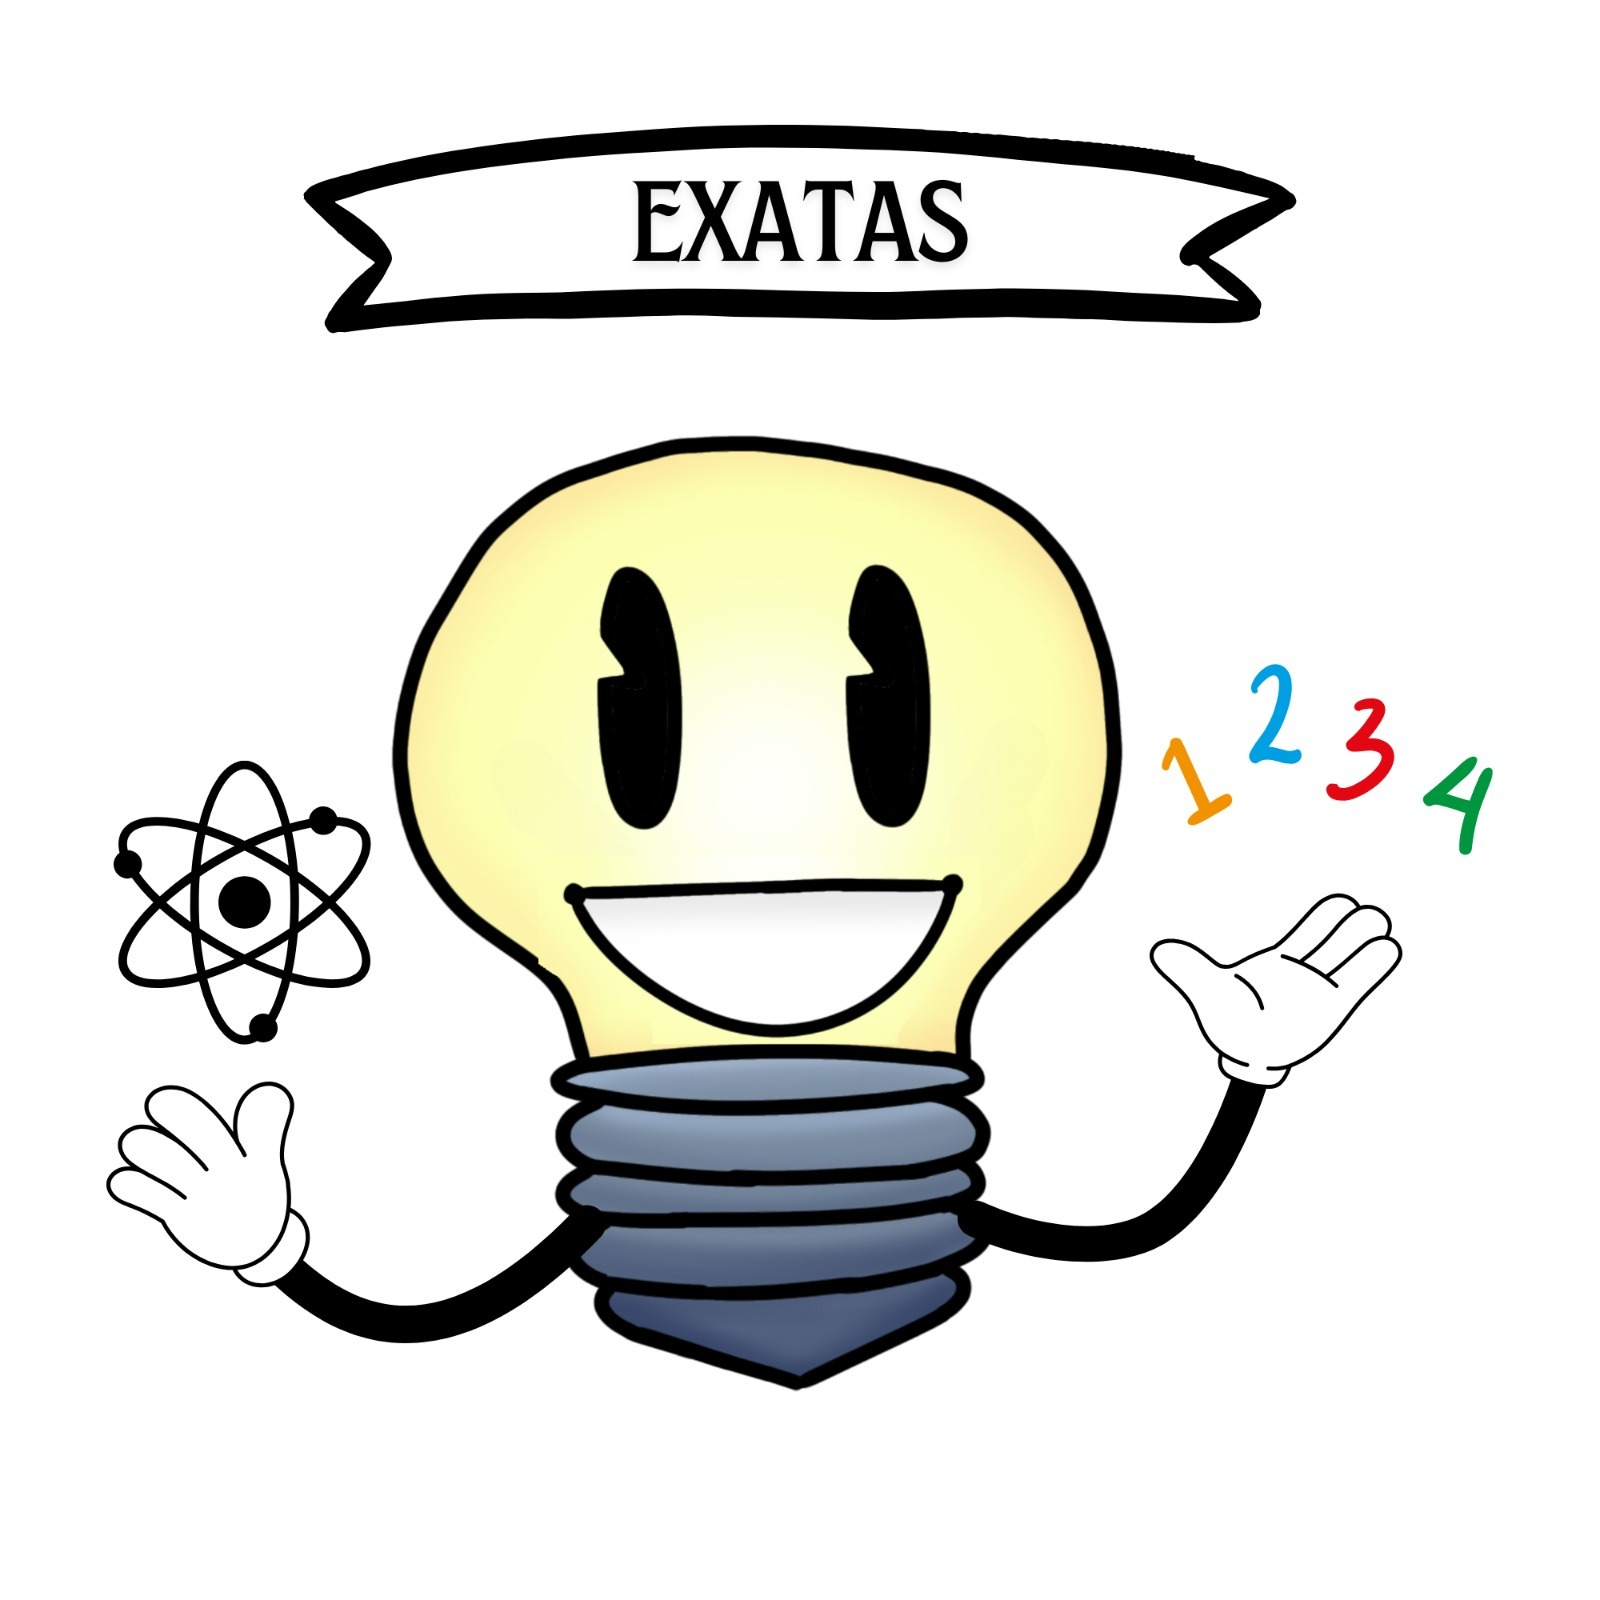
\includegraphics[width=2cm]{exata.jpg}}}  % Esquerda
\fancyhead[R]{\hspace{1cm}\raisebox{-2.8cm}{
\includegraphics[width=4cm]{pei.jpg}}} % Direita


%\newtcolorbox{boxA}{
%	fontupper = \bf,
%	boxrule = 1.5pt,
%	colframe = white  % frame color
	%rounded corners
	% arc = 5pt   % corners roundness	
%}

\begin{document}
	\fontsize{10}{15}\selectfont
	\vspace*{1mm}
	
	% ========= SEÇÃO: ATIVIDADE EXPRESSÕES ALGÉBRICAS ==========
	\section*{}	
	\begin{tcolorbox}[colback=gray!10, colframe=black, boxrule=0.5mm, arc=4pt, title=\textbf{Orientações}]
		A atividade deverá ser entregue até o dia \textbf{30/04}, com todas as resoluções feitas de forma completa e detalhada. 		
		Capriche nos cálculos e nas justificativas — isso será valorizado!
	\end{tcolorbox}
	
	\section*{EXPRESSÕES ALGÉBRICAS} 
				
	\begin{enumerate}
		\item Para determinar seu lucro nas vendas do dia, em reais, Kátia usa a fórmula matemática:  
		\boxed{  L = 8 \cdot u + 4,20  }
		Sendo $L$, o lucro das vendas e $‘u’$ o número de unidades vendidas, qual o lucro de Kátia em um dia que ela vender 45 unidades do produto?
		
		\item Júnior é minerador de ouro. Certo dia teve que alugar uma máquina, cujo valor a pagar é calculado de acordo com a expressão do quadro abaixo. \boxed{  L = 280 \cdot D + 10 \cdot Q}
		Nessa expressão, $V$ corresponde ao valor a pagar, $D$ ao número de dias e $Q$ aos quilômetros rodados. Se, Júnior, alugou por 7 dias e rodou 100 quilômetros, o valor a pagar pelo aluguel será:
		
		\item
		Na escola de Ariel, para cada disciplina são realizadas duas provas por conteúdo, quatro atividades, um trabalho e uma prova final em cada bimestre. Os pesos de cada componente na composição da média bimestral são:	\vspace*{-3mm}	
		\begin{center}
		20\% para cada prova (P1 e P2);	
			
		5\% para cada atividade (A1, A2, A3 e A4);	
			
		10\% para o trabalho (T);		
		
		30\% para a prova final (PF).
		\end{center} \vspace*{-5mm}		
		A média bimestral é calculada pela expressão: \\
		\boxed{ M = 0,2 \cdot P1 + 0,2 \cdot P2 + 0,05 \cdot A1 + 0,05 \cdot A2 + 0,05 \cdot A3 + 0,05 \cdot A4 + 0,1 \cdot T + 0,3 \cdot PF }
			
		Sabendo que Ariel obteve, respectivamente, as seguintes notas:
		P1 = 3, P2 = 6, A1 = 8, A2 = 7, A3 = 5, A4 = 9, T = 7 e PF = 8, qual será sua média bimestral?
		
		\item  Na expressão $x^2 + 5\cdot x - 8\cdot x \cdot y$. Calcule quando $x$ e $y$ assumir os valores: 
		\vspace{-5mm}
		\begin{multicols}{4}
			\begin{enumerate}[]
				\item $x = 2 $ \\ $y = 2 $
				\item $x = 5 $ \\ $ y = -2 $
				\item $x = -3$ \\ $ y = 4 $
				\item $x = 2^3$ \\ $ y = 3^2 $
			\end{enumerate}
		\end{multicols}
		
		\item O IMC (Índice de Massa Corporal) de uma pessoa adulta é calculado dividindo o seu peso pela altura elevada ao quadrado, usando-se a expressão \boxed{IMC = \frac{peso(kg)}{(altura(m))^2}} . Se a altura de Alana é 1,5m e ela pesa 72kg, então, o seu IMC de acordo com essa expressão é quanto? Qual sua classificação de acordo com o resultado do cálculo do IMC?
		
		\item Escreva a expressão algébrica que representa a área e o perímetro da seguinte figura: 
		\begin{center}
			\begin{tikzpicture}[scale=0.4]
				% Pontos
				\coordinate (A) at (0,0);
				\coordinate (B) at (0,6);
				\coordinate (C) at (4,6);
				\coordinate (D) at (8,0);
				
				% Linhas
				\draw [thick] (A) -- (B) -- (C) -- (D) -- (A);
				
				% Marcação de medidas
				\draw [decorate,decoration={brace,amplitude=8pt}] (A) -- (B) node[midway,left=8pt] {\small 6};
				\draw [decorate,decoration={brace,amplitude=8pt}] (B) -- (C) node[midway,above=8pt] {\small $x$};
				\draw [decorate,decoration={brace,amplitude=8pt}] (C) -- (D) node[midway,right=8pt] {\small $y$};
				\draw [decorate,decoration={brace,mirror,amplitude=8pt}] (A) -- (D) node[midway,below=8pt] {\small $x+8$};
				
			\end{tikzpicture}
		\end{center}
		Calcule o valor da área e do perímetro quando $x=3$ e $y=10$		
	\end{enumerate}			
\end{document}
